%!TEX root = main.tex
\chapter{Background}

\section{Reflection}
Our theoretical background for reflection.
\subsection{MIRROR.eu model}

\begin{figure}[h!]
\label{logo}
\centering
	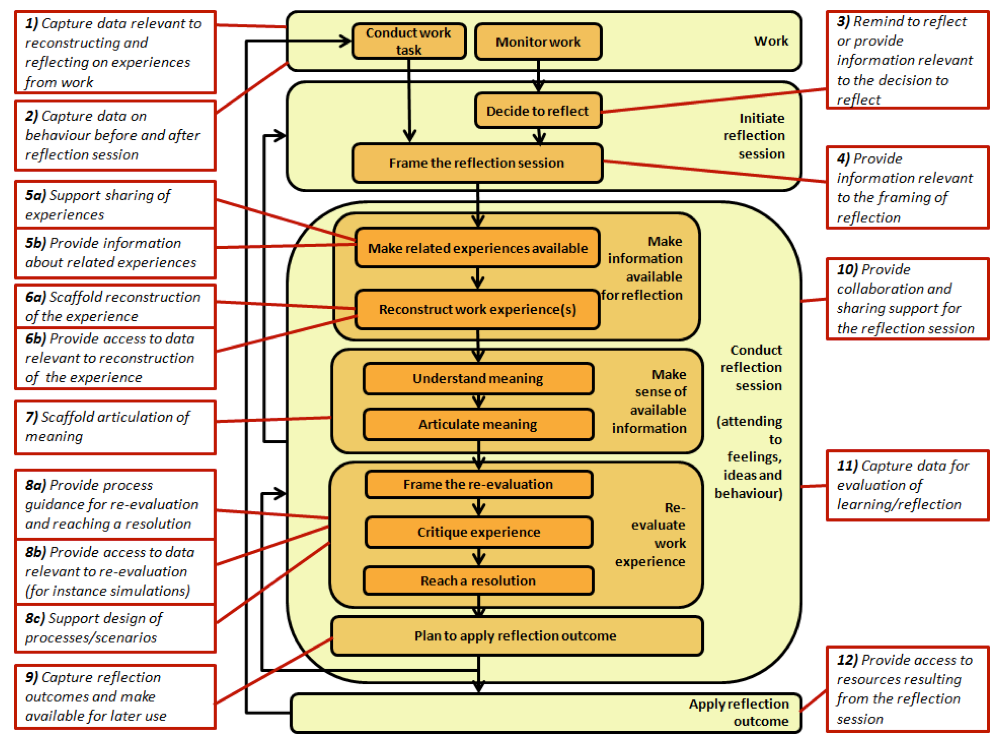
\includegraphics[width=\textwidth]{mirror}
\caption{MIRROR model}
\end{figure}
The MIRROR model is a work on how to incorporate reflection in to the daily rutine at work.

%\subsection{Birgits PHD}
% PhD: http://www.idi.ntnu.no/research/doctor_theses/birgitkr.pdf  .

\section{Agile development}
Theoretical background about agile development. Normaly a project is divided into milestones, these milestones will then again be divided into issues and weighted on how much work is required to finish working on each of them.

\begin{quotation}
Individuals and interactions over processes and tools
Working software over comprehensive documentation
Customer collaboration over contract negotiation
Responding to change over following a plan

That is, while there is value in the items on
the right, we value the items on the left more.

\em Manifesto for Agile Software Development
\end{quotation}

\begin{figure}[h!]
\label{logo}
\centering
	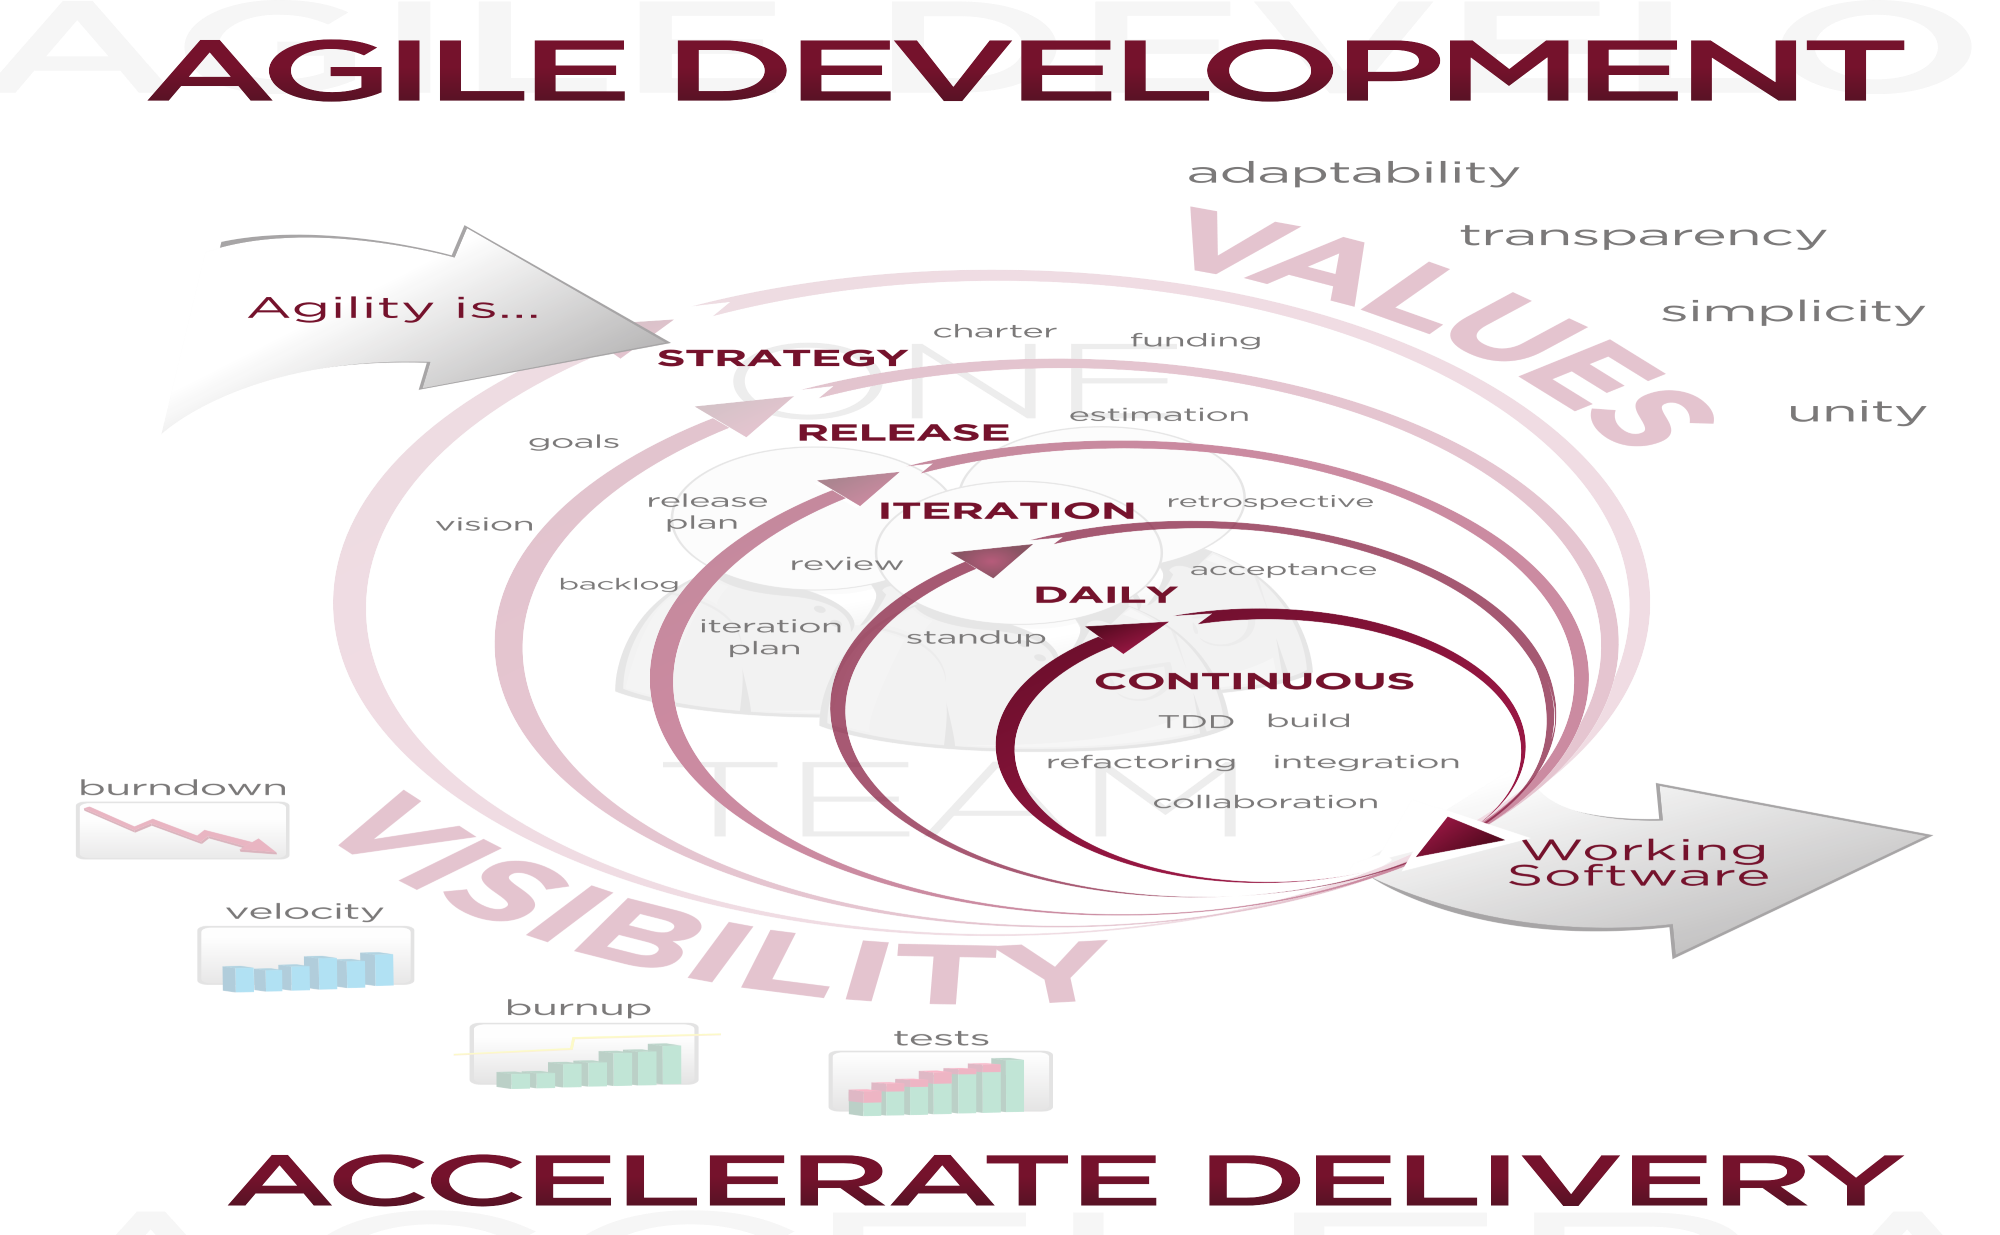
\includegraphics[width=\textwidth]{agile_model}
\caption{Agile software development poster}
\end{figure}

The poster above represents the different iterations a team of developeres iterates through when using agile development meothodology.

\subsection{Scrum}
Scrum is a type of agile development, it has set intervalls(normally 2 to 4 weeks) for each milestone with each milestone containing about the same amount of work.

\begin{figure}[h!]
\label{logo}
\centering
	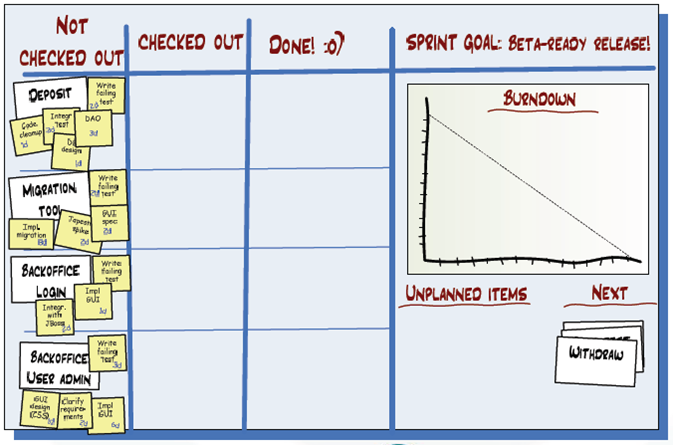
\includegraphics[width=\textwidth]{scrumboard}
\caption{Example of scrum board}
\end{figure}

A scrumboard as shown above is used for each milestone to show which issues have been started on and who is working on which feature. The chart to the right is a burndown chart, stating how many hours the team has to work inorder to complete on time.